%
% File naaclhlt2013.tex
%

\documentclass[11pt,letterpaper]{article}
\usepackage{naaclhlt2013}
\usepackage{times}
\usepackage{graphicx}
\usepackage{latexsym}
\usepackage{listings}
\usepackage{algorithm}
\usepackage[noend]{algpseudocode}

\newlength{\alglabelwidth}
\newcommand{\alginput}[1]{%
\par\noindent%
\settowidth{\alglabelwidth}{\emph{Output:}}%
\makebox[\alglabelwidth][l]{\emph{Input:}} \begin{tabular}[t]{l} #1 \end{tabular}}
\newcommand{\algoutput}[1]{%
\par\noindent%
\settowidth{\alglabelwidth}{\emph{Output:}}%
\makebox[\alglabelwidth][l]{\emph{Output:}} \begin{tabular}[t]{l} #1 \end{tabular}}
\newcommand{\algprecond}[1]{%
\par\noindent\textit{Initialization/Precondition: #1}}


\lstset{basicstyle=\ttfamily\footnotesize,       % the size of the fonts that are used for the code
		numbers=left,                   % where to put the line-numbers
		numberblanklines=false
		numbersep=1em,                  % how far the line-numbers are from the code
		basewidth=0.52em,
		tabsize=4,  		% sets default tabsize to 2 spaces
		xleftmargin=\leftmargini
      }
\renewcommand*\thelstnumber{\the\value{lstnumber}:}
% END lstlisting environments

\lstnewenvironment{sql}[1][]{\lstset{language=SQL,gobble=4,emphstyle=\textit,#1}}{}


\setlength\titlebox{6.5cm}    % Expanding the titlebox

\title{Large-scale Statistical Text Analytics in RDBMS\Thanks{This
    submitting for double-blind reviewing.}}

\author{Kun Li, Christan Grant, Daisy Zhe Wang\\
	    University of Florida\\
	    111 Anywhere Street\\
	    Gainesville, FL 32608, USA\\
	    {\tt kli@cise.ufl.edu}
	  \And
	Sunny Khatri, George Chitouras\\
  	Greenplum/EMC\\
  	900 Main Street\\
	    Gainesville, FL 32608, USA\\
  {\tt george.chitouras@emc.com}}

\date{}

\begin{document}
\maketitle
\begin{abstract}
Many companies keep large stores of text files and user logs in relational databases.
For these companies to perform analyics on these datasets, these companies must perform 
expensive transfers between databases and analyitic systems.
Additionally, may popular text analytics packages do not scale to production sized datasets.
In this paper, we introduce MADText, an open source in-database statistical text analytics module.
This module is a part of MADLib, a open source library for scalable in-database text analytics. 
%which is an open source project for statistical and parallel library for in-database analytics.  
We show that we can use the declarative SQL interface instead of procedural code to perform 
conditional random field based part-of-speech tagging and named-entity resolution. 
We design schema to store single and two-state features.
By using these novel schemas, we avoid costly feature re-compution for the same token over and over again.  
As far as we know, MADText is the first toolkit for statistical text analysis in relational database management systems (RDBMS).  
In the application level, we can support part-of-speech tagging(POS), named entity resolution and entity detection.  
We show that our package is linearly scalable and outperform the state of art packages by caching and avoiding costly re-compution.
%Lastly, we show that MADText can do nearly real time hot topics discovery for each statesof USA using streaming Tweets.
\end{abstract}

\section{Introduction}

MapReduce systems e.g. Google's MapReduce, Apache Hadoop have gain more and more popularity since it was invented. All big companies are running hundreds of MapReduce jobs each day and each jobs contains terabytes of data.  These data can be structured data such as transaction data and unstructured data such as natural text data. 
Traditional business intelligence has to pull out of the data from databases into other massive data warehouses(OLAP) to analyze the data. 
However, it is time consuming to pull out the data from the databases, use other external tools to do data analysis, and then write the results back into database.
No doubt, the database is the place for data and also parallel database has the massive parallel processing engine. 
So besides the data accounting functionality of relational database management systems (RDBMS), in-database analytics functionality has been pushing into RDBMS to enable a deep insight into the data by the database vendors.  From one side, data don’t need to move back and forth.
On the other side, the database embarrassingly parallel processing engine can be leveraged to handle Big Data. 
Motivated by these arguments, database researchers and database vendors are trying to make these practical which leads to the MADlib project. MADlib is an open source library for scalable in-database analytics. It provides parallel implementation of machine learning algorithms.
Text analytics has gains has more and more attention due to huge amount of text data generated from web, social networks every day.
Understanding this natural text data is crucial to business decision and even political campaign. 
Companies are analyzing text data to discover the popularity of specific topic and do sentiment analysis over certain products.
We enable statistical text analysis in parallel databases using linear chain conditional random filed, which is state of art 
probabilistic graphical model on real natural language processing tasks such as part of speech tagging and named entity recognition.
We design a novel schema, that enables us to 
perform one time feature extraction and avoid re-computing the features for one token. 
We are able to use the falicity provided by a RDMBS to achieve the parallel CRF learning and inference for NLP tasks.

\section{Related Work}
Our work is inspired by a description of a unified architecture for in-RDBMS analytics \cite{Feng:2012:TUA:2213836.2213874}.
The paper points out that most of the machine learning algorithms confined to a unified architectures in RDBMS\@.
Essentially, the majority of machine learning algorithms can be reduced to a maximum likelihood objective function. % Multiple runs
The gradient vector and log likelihood can be calculated in parallel using user-defined aggregates supported in most of the RDBMS.
%User defined aggregates is MapReduce like framework to do parallel processing.
It also defines a driver function that manages the multi-pass optimization process until convergence criterion is met.
There are several implementations conditional random fields and but only a few large scale implementations for NLP tasks 

such as PCRFs \cite{phan2004flexcrfs}. 

SystemT\cite{chiticariu2010systemt}.

GATE \cite{Cunningham2011a}.

Wang's work on CRF inference Limited-memory BFGS We design novel relational schemas to store all the inputs, features, and outputs.

\section{Linear-chain CRF for IE in RDBMS}
Part-of-speech tagging (POS), also called grammatical tagging and word-category disambiguation is the process of assigning 
a part of speech to each word in a sentence. POS has been widely used in information retrieval and text to speech. 
There are two distinct methods for 
POS task, rule-based and stochastic.
In rule-based method, large collection of rules are defined to indentify the tag. Stochastic methods are based on 
probabilistic graphic models such as hidden markov models and conditional random fields. In practice, 
conditional random fields are approved to achieve the state of art accuracy.


\subsection{In-database Implementation}
We use SQL clauses to generate all features for text. Any features in the state of art packages can be extracted using one single SQL clause.
All the features can be stored in two schemas. M and R. M table stores the features involves two states. R table store all the single state features.
After the feature extraction, we use user-defined aggregates to calculate the gradient and log-likelihood parallel using the transition function.
We also implement the LBFGS in database. Difference between in database and in memory implementation.
  
\subsection{System Architecture}
\begin{center}
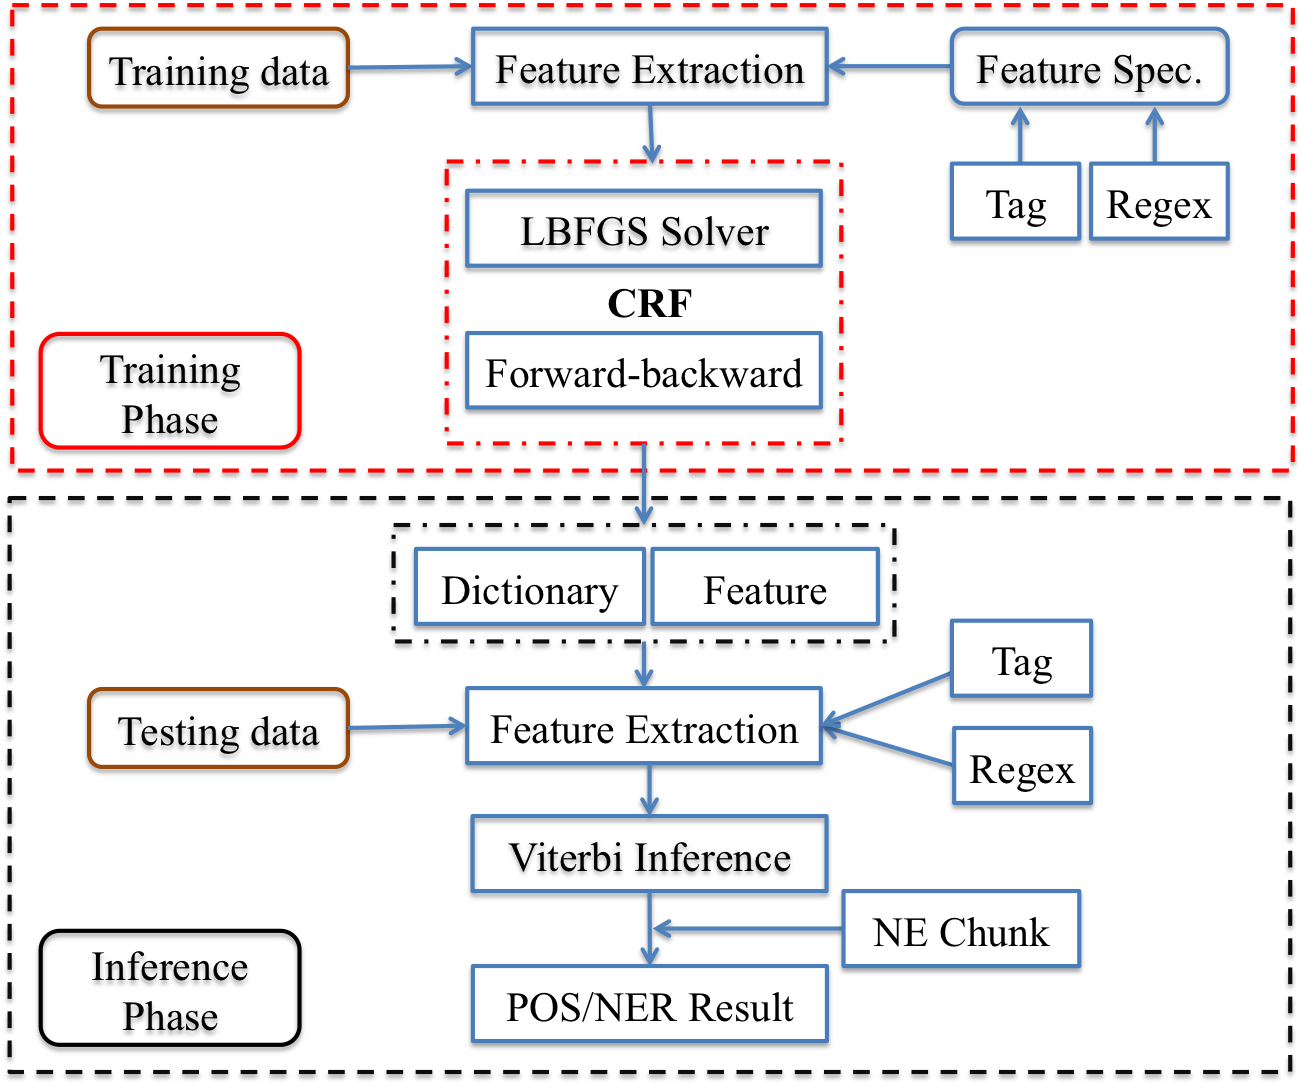
\includegraphics[height=15em]{system.png}
\end{center}

\subsection{Feature Extraction Using SQLs}
Text feature extraction is a step in most statistical text analysis methods.
We are able to implement all of the seven types of features used in POS and NER using exactly seven 
SQL statements. These features are: 
(1) dictionary features: does this token exist in a provided dictionary? 
(2) regex features: does this token match a provided regular expression? 
(3) edge features: is the label of a token correlated with the label of a previous token? 
(4) word features: does this the token appear in the training data?
(5) unknown feature: does this token appeared in the training data below certain threshold? 
(6) start feature: is this token the first in the token sequence? and 
(7) end feature: is this token the last in the token sequence?

There are many advantages for extracting features using SQLs.  
Compared with procedure language, SQL is much more easier to understand. 
It turns out that each type of feature can be extracted out using exactly one SQL statement, 
which make the feature extraction code extremely succinct.  
From a pedagogical point of view, it is much easier to teach text feature extraction using our SQL feature extraction code.
Secondly, SQLs are naïvely parallel due to sets operations. 
Lastly, we computed features for each distinct token, which avoid re-computing the features for the same token.  
$SQL_1$:\\
\begin{lstlisting}[language=SQL,gobble=4]
    SELECT doc2.start_pos, doc2.doc_id, 'E.', 
           ARRAY[doc1.label, doc2.label]
    FROM   segmenttbl doc1, segmenttbl doc2
    WHERE  doc1.doc_id = doc2.doc_id AND 
           doc1.start_pos+1 = doc2.start_pos
\end{lstlisting}

%\item 
$SQL_2$:\\
\begin{lstlisting}[language=SQL,gobble=4]
    SELECT start_pos, doc_id, 'R_' || name, 
           ARRAY[-1, label]
    FROM  regextbl, segmenttbl
    WHERE seg_text ~ pattern
\end{lstlisting}
%\end{itemize}

\paragraph{Build the feature dictionary and assign each feature with a unique feature id}
%\begin{itemize}
%\item 
$SQL_3$\\ 
\begin{lstlisting}[language=SQL,gobble=4]
    INSERT INTO tmp_featureset(f_name, feature) 
    SELECT DISTINCT f_name, feature
    FROM   tmp1_feature;
    INSERT INTO featureset(f_index, f_name, feature) 
    SELECT nextval('seq')-1, f_name, feature
    FROM   tmp_featureset;
\end{lstlisting}
%\end{itemize}

\paragraph{Generate sparse\_r table}
%\begin{itemize}
%\item $SQL_3$\\ 
\begin{lstlisting}[language=SQL,gobble=4]
    INSERT INTO rtbl(start_pos,doc_id,feature)
    SELECT start_pos, doc_id, 
           array_cat(fset.feature, 
		     ARRAY[f_index,start_pos, 
		     CASE 
           WHEN tmp1_feature.feature=fset.feature 
           THEN 1
		     ELSE 0 END] )
    FROM   tmp1_feature, featureset fset
    WHERE  tmp1_feature.f_name = fset.f_name AND 
           fset.f_name <> 'E.';
\end{lstlisting}
%\end{itemize}


\subsection{Parallel Linear-chain CRF Training}
\begin{algorithm} 
\caption{CRF training$(z_{1:M})$} \label{alg:CRF training}
\alginput{Observation set $z_{1:M}$,\\
convergence criterion $\mathit{Convergence}()$,\\
start strategy $\mathit{Start}()$,\\
initialization strategy $\mathit{Initialization}()$,\\
transition strategy $\mathit{Transition}()$,\\
finalization strategy $\mathit{Finalization}()$}
\algoutput{Coefficients $w \in R^N$}
\algprecond{$iteration = 0, diag = 1$}
\begin{algorithmic}[1]
\State $w_{new} \gets \mathit{Start}(z_{1:M})$
\Repeat
        \State $w_{old} \gets w_{new}$
        \State $\mathit{state} \gets \mathit{Initialization}(w_{new})$
\For{$m \in 1..M$} \Comment{Single entry in the observation set}
\State $\mathit{state} \gets \mathit{Transition}(\mathit{state}, z_m)$
                \Comment{Computing gradient and log-likelihood.}
\EndFor
\State $w_{new} \gets Finalization(\mathit{state})$ \Comment{Mainly invoke L-BFGS convex solver}
\Until{$Convergence(w_{new}, g_{new}, \mathit{iteration})$}
    \State \Return $w_{new}$
\end{algorithmic}
\end{algorithm}

\paragraph{Programming Model.}
We provide above the algorithm of parallel CRF training strategy, in the fashion of the selected programming model supported by MADlib (mainly user-defined aggregate).

\paragraph{Parallelism.}
The outer loop is inherently sequential over multiple iterations.
The iteration $n+1$ takes the output of iteration $n$ as input, so on so forth until the stop criterion is satisfied.
The inner loop which calculates the gradient and log-likelihood for each document is data-parallel.
Simple model averaging are used to merge two states.
A merge function is not explicitly added to the pseudocode for simplicity.
The finalization function invokes the L-BFGS convex solver to get a new solution. L-BFGS is sequential, but very fast.
Experiments show that the speed-up ration approaches the number of segments configured in the Greenplum database.

\paragraph{Convergence criterion.}
Usually, the following conditions are combined by AND, OR, or NOT.
\begin{enumerate}
    \item The norm of gradient divided by the norm of coefficient drops below a given threshold.
    \item The maximum number of iterations is reached.
    \item There could be more.
\end{enumerate}

\paragraph{Start strategy.}
In most cases, zeros are used unless otherwise specified.

\paragraph{Transition strategies.}
This function contains the logic of computing the gradient and log-likelihood for each tuple using the forward-backward
algorithm. The algorithms will be discussed in the following sections.

\begin{algorithm}
\caption{transition-lbfgs$(\mathit{state}, z_m)$} \label{alg:transition-lbfgs}
\alginput{Transition state $\mathit{state}$,\\
observation entry $z_m$,\\
gradient function $\mathit{Gradient}()$}
\algoutput{Transition state $\mathit{state}$}
\begin{algorithmic}[1]
    \State $\{state.g,state.loglikelihood\} \gets \mathit{Gradient}(\mathit{state}, z_m)$
        \Comment{using forward-backward algorithm to calculate gradient and loglikelihood}
    \State $\mathit{state}.num\_rows \gets \mathit{state}.num\_rows + 1$
    \State \Return $\mathit{state}$
\end{algorithmic}
\end{algorithm}


\paragraph{Merge strategies.}
The merge function simply sums the gradient and log-likelihood over all training documents
\begin{algorithm}
\caption{merge-lbfgs$(\mathit{state_1}, \mathit{state_2})$} \label{alg:merge-lbfgs}
\alginput{Transition state $\mathit{state_1}$,\\
Transition state $\mathit{state_2}$}
\algoutput{Transition state $\mathit{state_{new}}$}
\begin{algorithmic}[1]
    \State $\mathit{state_{new}}.g \gets \mathit{state_1}.g + \mathit{state_2}.g$
    \State $\mathit{state_{new}}.loglikelihood \gets \mathit{state_1}.loglikelihood + \mathit{state_2}.loglikelihood$
    \State \Return $\mathit{state_{new}}$
\end{algorithmic}
\end{algorithm}


\paragraph{Finalization strategy.}
The finalization function invokes the L-BFGS convex solver to get a new coefficent vector.\\

\begin{algorithm}
\caption{finalization-lbfgs$(state)$} \label{alg:CRF training}
\alginput{Transition state $state$,\\
LBFGS $\mathit{lbfgs}()$}
\algoutput{Transition state $state$}
\begin{algorithmic}[1]
        \State $\{state.g,state.loglikelihood\} \gets penalty(state.g,state.loglikelihood)$ \Comment{To avoid overfitting, add penalization}
        \State $\{state.g,state.loglikelihood\}\gets-\{state.g,state.loglikelihood\}$ \Comment{negation for maximization}
        \State LBFGS instance($state)$ \Comment{initialize the L-BFGS instance with previous state}
        \State instance.$lbfgs()$ \Comment{invoke the L-BFGS convex solver}
        \State instance.save\_state$(state)$ \Comment{save updated variables to the state for next iteration}
        \State \Return $state$
\end{algorithmic}
\end{algorithm}

Feeding with current solution, gradient, log-likelihood, etc., the L-BFGS will ouput a new solution.
To avoid overfitting, a penalization function is needed. We choose to penalize the log-likelihood with a spherical Gaussian weight prior.
Also, L-BFGS is to maximum objective, so we need to negate the gradient vector and log-likelihood to fit our needs in order minimize the log-likehood.

\paragraph{LBFGS Convex Optimization}
The limited-memory BFGS(L-BFGS) is the limited memory variation of the Broyden-Fletcher-Goldfarb-Shanno(BFGS) algorithm which
is the state of art of large scale non constraint convex optimization method.
We translate the in-memory Java implementation to C++ in-database implementation using Eigen support.
Eigen vector and Eigen matrix are used instead of the plain one dimentional and two dimentional arrays.
In the Java in-memory implementation, it defines many static variables defined and shared between the interations.
However, in the MADlib implementation, we define these variables in the state object.
Before each iteration of L-BFGS optimization, we need to initialize the L-BFGS with the current state object. 
At the end of each iteration, we need to dump the updated variables to the database state for next iteration.

\begin{lstlisting}[language=SQL,gobble=4]
    select crf_train_data('/path/to/trainingdata')
\end{lstlisting}

\begin{lstlisting}[language=SQL,gobble=4]
    select crf_train_fgen('train_data', 
    'regex','dic','featuretbl','feature_dic')
\end{lstlisting}

\begin{lstlisting}[language=SQL,gobble=4]
    select lincrf('featuretbl','sparse_r',
    'dense_m','sparse_m','f_size',45, 
    'feature_dic','feature',20)
\end{lstlisting}

\subsection{Parallel Linear-chain CRF Inference}
 The Viterbi algorithm is to find the top-k most likely labelings of a document 
for CRF models. 
We chose to implement a Python UDF that uses iterations to drive the Viterbi inference. 
In Greenplum, Viterbi can be run in parallel over different subsets 
of the document on a multi-core machine.

The $vcrf\_top\_label$ is implemented sequentially and each function call will finish labeling of one document. 
The inference is paralledl in the level of document. We use a SQL statment to drive the inference of all documents.
So, the CRF inference is naivelly parallel. 
\begin{lstlisting}[language=SQL,gobble=4]
    SELECT doc_id, vcrf_top1(m.score,r.score)
    FROM   mfactors as m ,rfactors as r
\end{lstlisting}

\paragraph{Inference}
\begin{lstlisting}[language=SQL,gobble=4]
    select crf_test_data('/path/to/testingdata')
\end{lstlisting}

\begin{lstlisting}[language=SQL,gobble=4]
    select crf_test_fgen('test_data','dic',
    'label','regex','feature','mtbl','rtbl')
\end{lstlisting}

\begin{lstlisting}[language=SQL,gobble=4]
    select vcrf_label('test_data', 
    'mtbl','rtbl','label','extraction')
\end{lstlisting}

\cite{DBLP:conf/icml/LaffertyMP01}
\cite{DBLP:journals/scholarpedia/Viterbi09}
\cite{DBLP:journals/siamjo/MoralesN00}
\cite{DBLP:journals/coling/DeRose88}
\cite{DBLP:conf/naacl/ShaP03}
\cite{DBLP:journals/coling/MarcusSM94}


%\begin{thebibliography}{}
%$\[
%V(i,y) =
%\begin{cases}
%\max_{y^\prime}(V(i-1,y^\prime)) + \textstyle \sum_{k=1}^K \lambda_kf_k(y,y^\prime,x_i), & \text{if } i\ge0 \\
%0, & \text{if } i=-1.
%\end{cases}
%\]$

\subsection{Entity Detection}

\section{Experiments and Results}
In order to evaluate the performance and scalability of the linear-chain CRF learning and inference on Greenplum,
we conduct experiments on various data sizes over on a 32-core machine with 2T hard drive and 64G memory.
We use CoNLL2000 dataset containing 9000 tagged sentences for learning. This dataset is labeled with the Treebank II
as the tag set. We truncated the dataset into 6 datasets containing 1k, 2k, 4k, 6k, 8k, 9k sentences respectively.
To evaluate the inference performance, we extract 1 million sentences from news and truncated the inference datasets into 5 dataset contains 100k, 200k, 400k, 600k, 800k, 1000k sentences.

Linear-chain CRF Training:\\
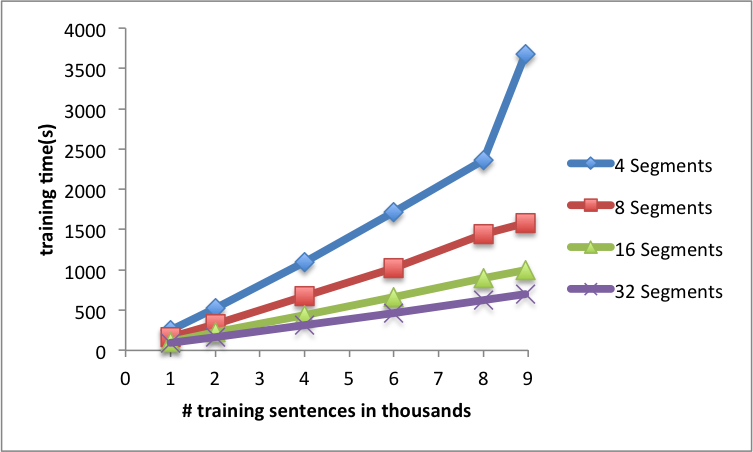
\includegraphics[height=11em]{training}
Linear-chain CRF Inference:\\
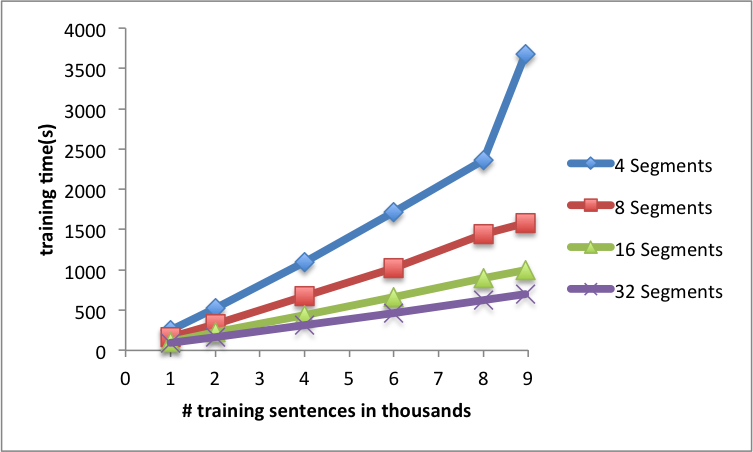
\includegraphics[height=11em]{training}

\section{User Case: Tweet Analysis}
\label{sec:blind}

\section{Conclusion}

\section*{Acknowledgments}
Christan Grant is funded by a National
Science Foundation Graduate Research Fellowship under Grant No. DGE-0802270.
This work was supported by a gift from EMC Greenplum.

\bibliographystyle{plain}
\bibliography{citation}

\end{document}
